\documentclass[aspectratio=169]{../latex_main/tntbeamer}  % you can pass all options of the beamer class, e.g., 'handout' or 'aspectratio=43'
\usepackage{dsfont}
\usepackage{bm}
\usepackage[english]{babel}
\usepackage[T1]{fontenc}
%\usepackage[utf8]{inputenc}
\usepackage{graphicx}
\graphicspath{ {./figures/} }
\usepackage{algorithm}
\usepackage[ruled,vlined,algo2e,linesnumbered]{algorithm2e}
\usepackage{hyperref}
\usepackage{booktabs}
\usepackage{mathtools}

\usepackage{amsmath,amssymb}

\DeclareMathOperator*{\argmax}{arg\,max}
\DeclareMathOperator*{\argmin}{arg\,min}

\usepackage{amsbsy}
\newcommand{\vect}[1]{\bm{#1}}
%\newcommand{\vect}[1]{\boldsymbol{#1}}

\usepackage{pgfplots}
\pgfplotsset{compat=1.16}
\usepackage{tikz}
\usetikzlibrary{trees} 
\usetikzlibrary{shapes.geometric}
\usetikzlibrary{positioning,shapes,shadows,arrows,calc,mindmap}
\usetikzlibrary{positioning,fadings,through}
\usetikzlibrary{decorations.pathreplacing}
\usetikzlibrary{intersections}
\pgfdeclarelayer{background}
\pgfdeclarelayer{foreground}
\pgfsetlayers{background,main,foreground}
\tikzstyle{activity}=[rectangle, draw=black, rounded corners, text centered, text width=8em]
\tikzstyle{data}=[rectangle, draw=black, text centered, text width=8em]
\tikzstyle{myarrow}=[->, thick, draw=black]

% Define the layers to draw the diagram
\pgfdeclarelayer{background}
\pgfdeclarelayer{foreground}
\pgfsetlayers{background,main,foreground}

% Requires XeLaTeX or LuaLaTeX
%\usepackage{unicode-math}

\usepackage{fontspec}
%\setsansfont{Arial}
\setsansfont{RotisSansSerifStd}[ 
Path=../latex_main/fonts/,
Extension = .otf,
UprightFont = *-Regular,  % or *-Light
BoldFont = *-ExtraBold,  % or *-Bold
ItalicFont = *-Italic
]
\setmonofont{Cascadia Mono}[
Scale=0.8
]

% scale factor adapted; mathrm font added (Benjamin Spitschan @TNT, 2021-06-01)
%\setmathfont[Scale=1.05]{Libertinus Math}
%\setmathrm[Scale=1.05]{Libertinus Math}

% other available math fonts are (not exhaustive)
% Latin Modern Math
% XITS Math
% Libertinus Math
% Asana Math
% Fira Math
% TeX Gyre Pagella Math
% TeX Gyre Bonum Math
% TeX Gyre Schola Math
% TeX Gyre Termes Math

% Literature References
\newcommand{\lit}[2]{\href{#2}{\footnotesize\color{black!60}[#1]}}

%%% Beamer Customization
%----------------------------------------------------------------------
% (Don't) Show sections in frame header. Options: 'sections', 'sections light', empty
\setbeamertemplate{headline}{empty}

% Add header logo for normal frames
\setheaderimage{
	% 
\includegraphics[height=\logoheight]{figures/TNT_darkv4.pdf}
	
\includegraphics[height=\logoheight]{../latex_main/figures/luh_logo_rgb_0_80_155.pdf}
	% 
\includegraphics[height=\logoheight]{figures/logo_tntluh.pdf}
}

% Header logo for title page
\settitleheaderimage{
	% 
\includegraphics[height=\logoheight]{figures/TNT_darkv4.pdf}
	
\includegraphics[height=\logoheight]{../latex_main/figures/luh_logo_rgb_0_80_155.pdf}
	% 
\includegraphics[height=\logoheight]{figures/logo_tntluh.pdf}
}

% Title page: tntdefault 
\setbeamertemplate{title page}[tntdefault]  % or luhstyle
% Add optional title image here
%\addtitlepageimagedefault{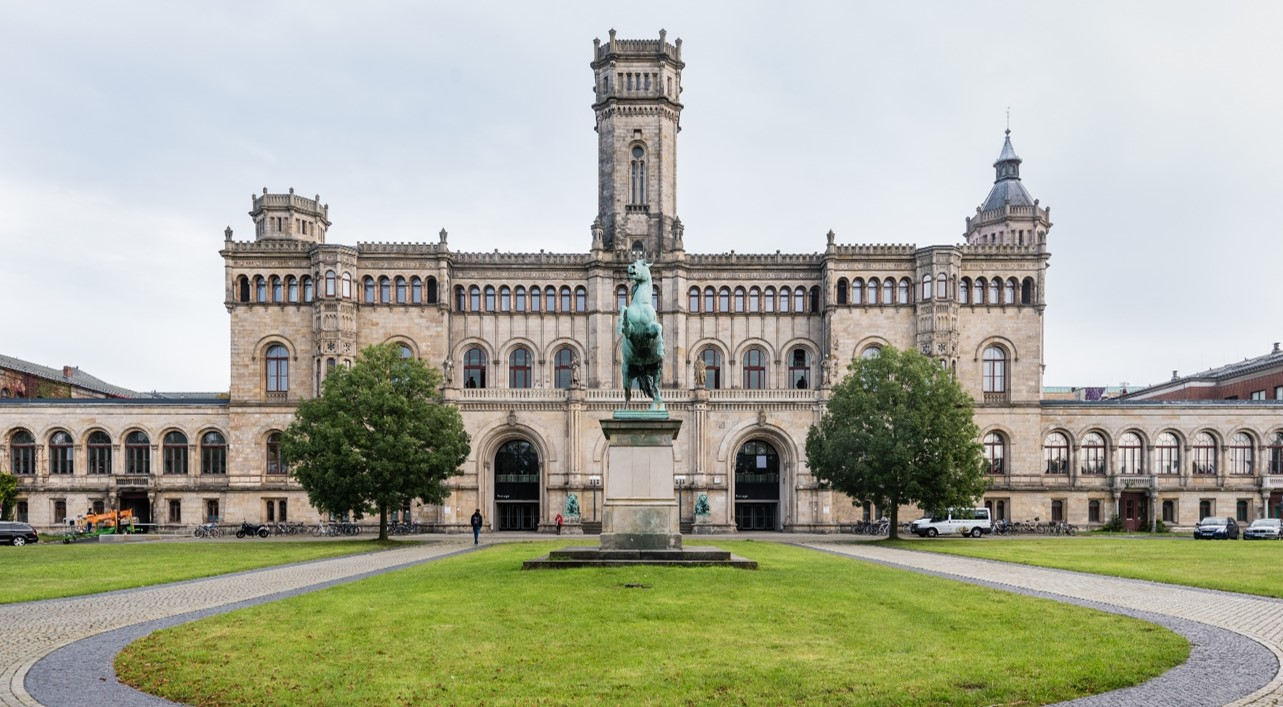
\includegraphics[width=0.65\textwidth]{figures/luh_default_presentation_title_image.jpg}}

% Title page: luhstyle
% \setbeamertemplate{title page}[luhstyle]
% % Add optional title image here
% \addtitlepageimage{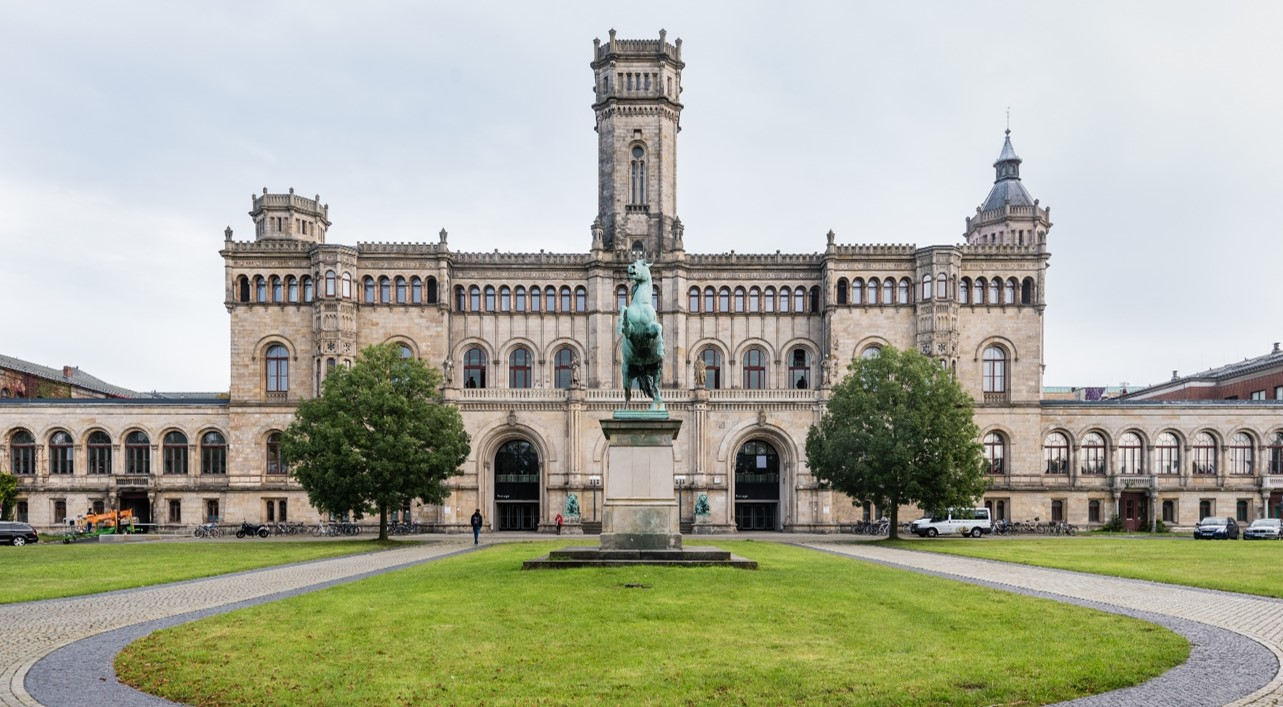
\includegraphics[width=0.75\textwidth]{figures/luh_default_presentation_title_image.jpg}}

\author[Abedjan \& Lindauer]{Ziawasch Abedjan \& Marius Lindauer\\[1em]
	
\includegraphics[height=\logoheight]{../latex_main/figures/luh_logo_rgb_0_80_155.pdf}\qquad
	
\includegraphics[height=\logoheight]{../latex_main/figures/DBIS_Kurzlogo.png}\qquad

\includegraphics[height=\logoheight]{../latex_main/figures/TNT_darkv4}\qquad

\includegraphics[height=\logoheight]{../latex_main/figures/L3S.jpg}	}
\date{Summer Term 2022; \hspace{0.5em} {
\includegraphics[height=1.5em]{../latex_main/figures/Cc-by-nc-sa_icon.svg.png}}; based on \href{https://ds100.org/fa21/}{[DS100]}
}


%%% Custom Packages
%----------------------------------------------------------------------
% Create dummy content
\usepackage{blindtext}

% Adds a frame with the current page layout. Just call \layout inside of a frame.
\usepackage{layout}


%%% Macros
%\renewcommand{\vec}[1]{\mathbf{#1}}
% \usepackage{bm}
%\let\vecb\bm

\title[Introduction]{DS: Logistic Regression, Classification}
\subtitle{Decision boundaries}

\graphicspath{ {./figure/} }
%\institute{}


\begin{document}
	
	\maketitle
	\begin{frame}{Decision boundaries}
	    \begin{columns}
	        \begin{column}{.5\textwidth}
	            Consider our original single-feature model.\\
	            \bigskip
	            $P(Y=1|x) = \sigma (\theta_1 \cdot FG\_PCT\_DIFF)$\\
	            \bigskip
	            The grey dots are true observations from the 2017-18 NBA season.
	             
	        \end{column}
	        
	        
	        \begin{column}{.5\textwidth}
	                \begin{figure}
	                    \centering
	                    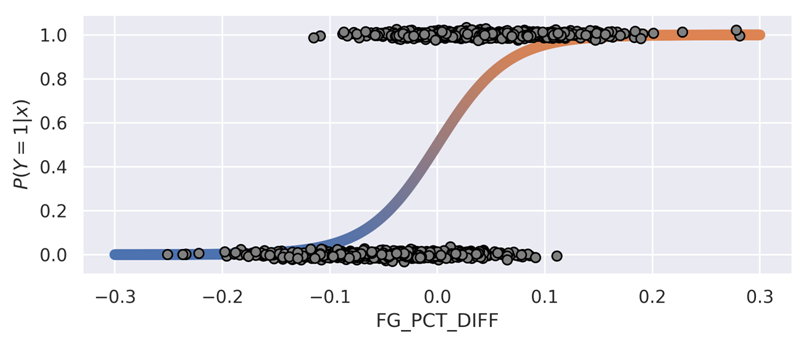
\includegraphics[scale=.55]{Bild33}\\
	                \end{figure}
	        \end{column}
	        
	    \end{columns}
	\end{frame}
	
	\begin{frame}{Decision boundaries}
	    \begin{columns}
	        \begin{column}{.5\textwidth}
	            If we pick a threshold, e.g. T = 0.3, we get a predicted class from probabilities.
	        \end{column}
	        
	        
	        \begin{column}{.5\textwidth}
	                \begin{figure}
	                    \centering
	                    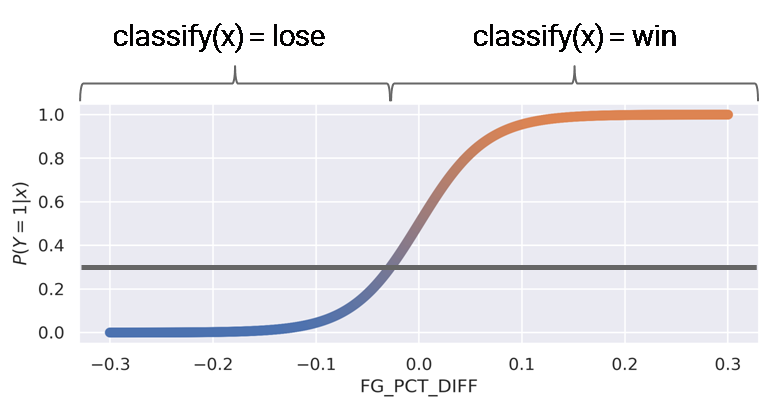
\includegraphics[scale=.55]{Bild34}\\
	                \end{figure}
	        \end{column}
	        
	    \end{columns}
	\end{frame}
	
	\begin{frame}{Decision boundaries }
	    \begin{columns}
	        \begin{column}{.5\textwidth}
	            If we pick a threshold, e.g. T = 0.3, we get a predicted class from probabilities.
	            \begin{itemize}
	                \item The effect is that x < xT predicts class 0, and x > xT predicts class 1.
	                \item $x_T$ is known as a decision boundary.
	                \begin{itemize}
	                    \item $x_T$ is a function of model parameters and T.

	                \end{itemize}
	            \end{itemize}
	        \end{column}
	        
	        
	        \begin{column}{.5\textwidth}
	                \begin{figure}
	                    \centering
	                    
\includegraphics[scale=.35]{Bild35}\\
	                \end{figure}
	        \end{column}
	        
	    \end{columns}
	\end{frame}
	
	
	\begin{frame}{Decision boundaries for 2D models}
	
	Now consider our “better” model, $ P(Y=1|x) = \sigma (\theta_0  + \theta_1 \cdot FG\_PCT\_DIFF + \theta_2 \cdot PF\_DIFF)$                                                    . It is drawn below with the thresholding line T = 0.3. What does its decision boundary look like?\\
        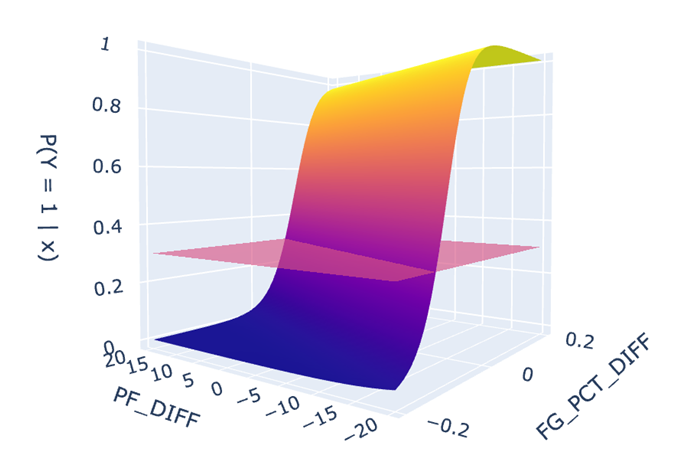
\includegraphics[scale=.5]{Bild36}
	     
	\end{frame}
	
	
	\begin{frame}{Decision boundaries for 2D models}
	
	Now consider our “better” model, $ P(Y=1|x) = \sigma (\theta_0  + \theta_1 \cdot FG\_PCT\_DIFF + \theta_2 \cdot PF\_DIFF)$                                                    . It is drawn below with the thresholding line T = 0.3. . The decision boundary is linear. \\
	
        \begin{figure}
            \centering
            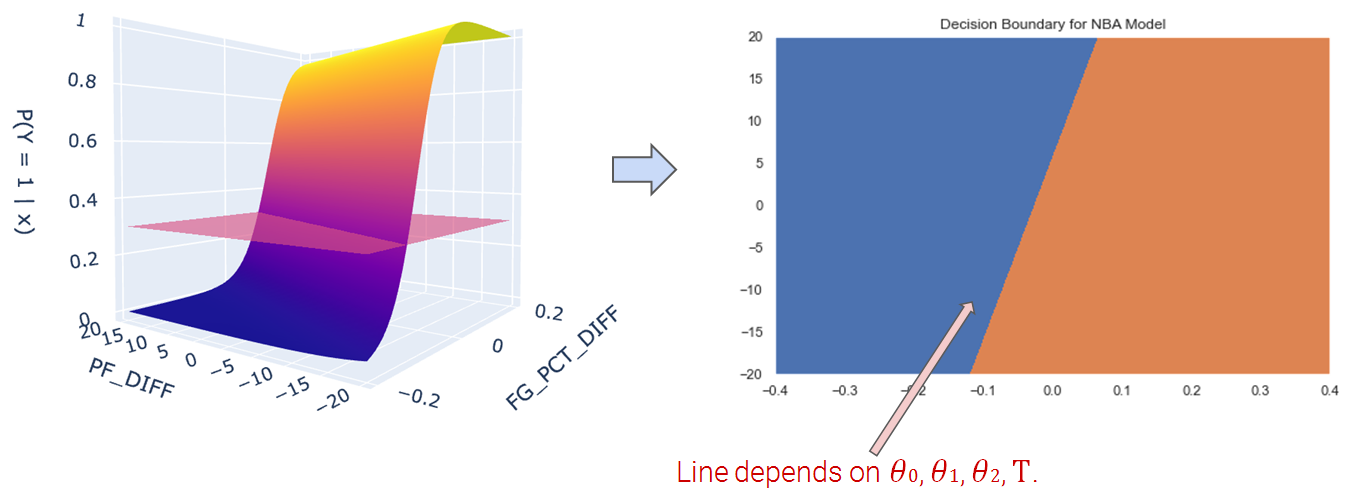
\includegraphics[scale=.35]{Bild37}
        \end{figure}
	     
	\end{frame}
	
	\begin{frame}{Decision boundaries for 2D models}
	Suppose we minimized mean cross-entropy loss to determine the optimal model parameters for this model, and found\\
	$P(Y=1|x) = \sigma (0.035 + 34.705\cdot FG\_PCT\_DIFF - 0.160\cdot PF\_DIFF)$\\
	\bigskip
	If we set T = 0.3, our decision boundary is \\
	$\sigma (0.035 + 34.705\cdot FG\_PCT\_DIFF - 0.160\cdot PF\_DIFF) = 0.3$\\
	\bigskip
	Which simplifies to
	%$0.035 + 34.705\cdot FG\_PCT\_DIFF - 0.160\cdot PF\_DIFF = \sigma^{-1}(0.3)$
	
        \begin{figure}
            \centering
            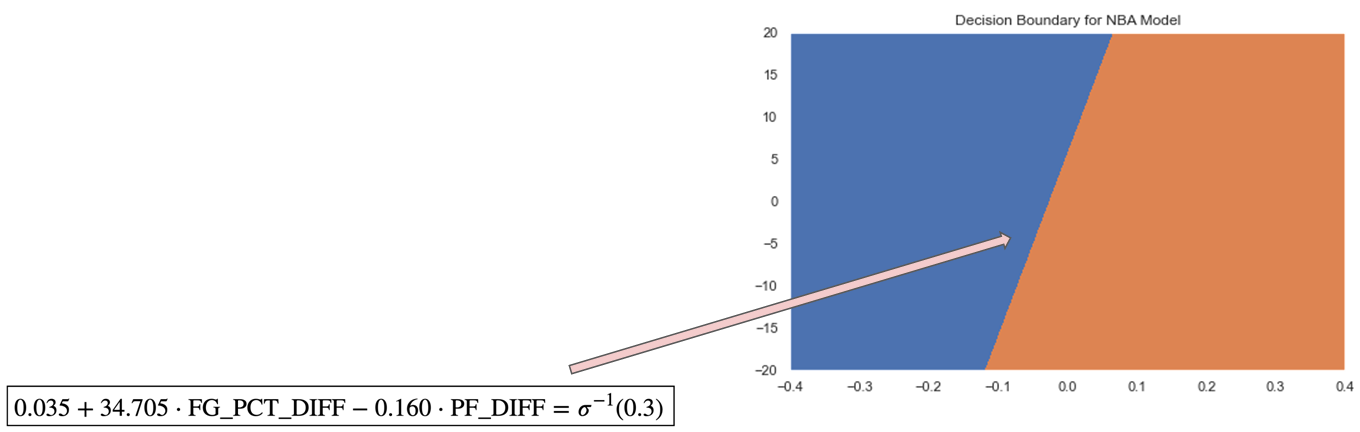
\includegraphics[scale=.25]{Bild38}
        \end{figure}
	     
	\end{frame}
	
	
	\begin{frame}{Decision boundaries for 2D models}
	If we overlay our true observations onto our decision boundary, we can get a rough sense of the accuracy of our model and the types of errors it makes.\\
	\begin{itemize}
	    \item Blue points in the orange region are false positives.
	    \item Orange points in the blue region are false negatives.
	\end{itemize}
	
        \begin{figure}
            \centering
            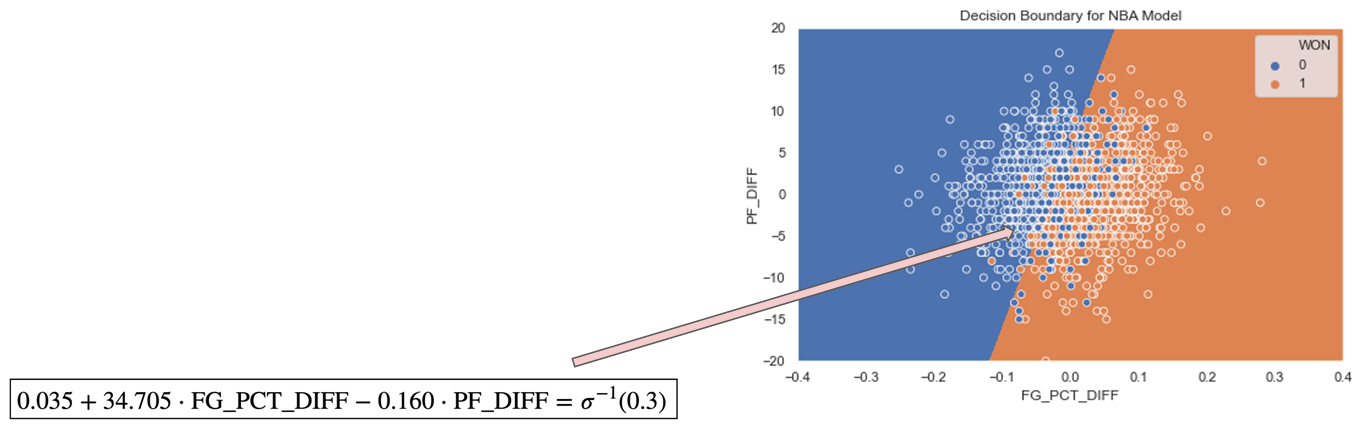
\includegraphics[scale=.35]{Bild39}
        \end{figure}
	     
	\end{frame}
	
	
\end{document}